%
% fdm.tex
%
% (c) 2020 Prof Dr Andreas Müller, Hochschule Rapperswil
%
\section{Finite Differenzen
\label{section:finite-differenzen}}
\rhead{Finite Differenzen}
Jedes Lösungsverfahren für partielle Differentialgleichungen muss die
unendlich vielen Freiheitsgrade, die eine Funktion
$u\colon\Omega\to\mathbb R$ enthalten kann, auf eine endlich Zahl von
Variablen reduzieren, für die sich ein Gleichungssystem aufstellen 
lässt, welches dann mit einer der früher studierten Methoden
gelöst werden kann.

%
% Gitter und Ableitungen
%
\subsection{Gitter und Ableitungen
\label{pde:subsection:gitter}}
Eine einfache Methode, die Funktion $u$ eine endliche Menge von Parametern
zu reduzieren, ist, nur die Werte in einzelnen Punkten des Gebietes 
$\Omega$ zu verwenden.
Als Beispiel betrachten wir ein Gebiet $\Omega\subset\mathbb R^2$
in der Ebene.
Dazu betrachten wir die Punkte
\[
x_{ik} = (ih_x, kh_y) \in \mathbb R^2
\qquad
i,k\in\mathbb Z,
\]
sie bilden ein Gitter $\Gamma$ mit Gitterkonstante oder Schrittweite
$h_x$ in $x$-Richtung und $h_y$ in $y$-Richtung.

Die Funktion $u(x,y)$ nimmt in den Punkten $x_{ik}$ die Werte
$u_{ik} = u(x_{ik})$ an.
Eine approximative Lösung der Differentialgleichung ist also
die Bestimmung der Werte $u_{ik}$ für die Punkte $x_{ik}$, die in
$\Omega$ liegen, für die also $x_{ik}\in\Omega$ gilt.
Dazu müssen jetzt die Randbedingungen und die Differentialgleichung
übersetzt werden in Gleichungen für die Unbekannten $u_{ik}$.

\subsubsection{Dirichlet-Randbedingungen}
Dirichlet-Randbedingungen geben die Werte auf dem Rand vor.
Liegt ein Punkt $x_{ik}$ des Gitters $\Gamma$ auf dem Rand $\partial\Omega$
von $\Omega$, dann geben die Dirichlet-Randbedingungen den Wert
dieser Variablen vor.
Es ist daher anzustreben, das Gitter $\Gamma$ so zu wählen, dass 
der Rand durch Gitterpunkte verläuft.
Ein gekrümmter Rand wird daher im Allgmeinen durch eine Kurve durch
die Gitterpunkte approximiert werden müssen.

\subsubsection{Erste Ableitungen}
\begin{figure}
\centering
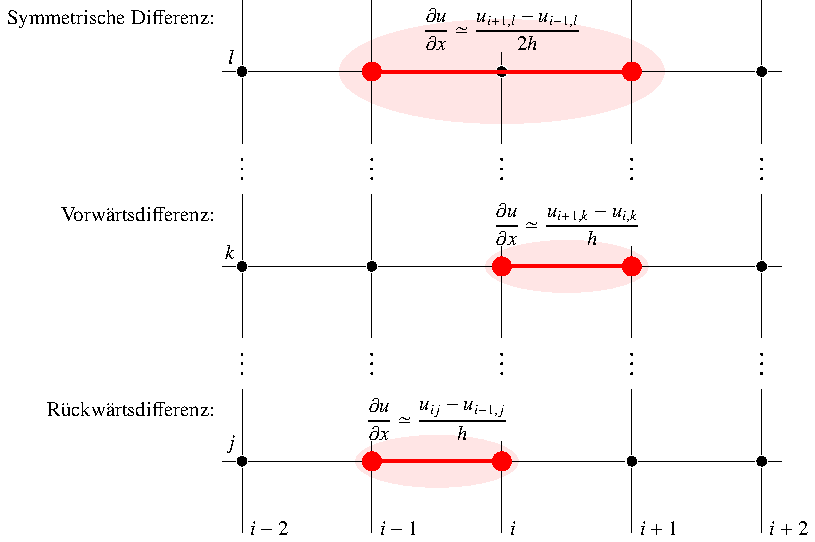
\includegraphics{chapters/70-pde/images/derivatives.pdf}
\caption{Approximation der ersten Ableitung mit verschiedenen
Differenzausdrücken
\label{buch:pde:1abldiff}}
\end{figure}
Die naheliegenste Approximation für die Differentialgleichung besteht
darin, die Ableitungen durch Differenzenquotienten zu ersetzen (siehe 
Abbildung~\ref{buch:pde:1abldiff}).
Mit der oben eingeführten Notation können die ersten Ableitungen durch
die sogenannten {\em Vorwärtsdifferenzen}
\index{Vorwärtsdifferenz}%
\begin{align}
\frac{\partial u}{\partial x} (x_{ik}) 
&\simeq
\frac{u(x_{i+1,k}) - u(x_{ik})}{h_x}
&
&\text{und}
&
\frac{\partial u}{\partial y} (x_{ik}) 
&\simeq
\frac{u(x_{i,k+1}) - u(x_{ik})}{h_y}
\label{chapter:pde:approx1st}
\end{align}
approximiert werden (Abbildung~\ref{buch:pde:1abldiff} Mitte).
Die Genauigkeit der Approximation kann offenbar verbessert werden, 
indem $h_x$ und $h_y$ verkleinert werden.

Der Fehler der Approximation~\eqref{chapter:pde:approx1st} ergibt sich
aus dem Mittelwertsatz der Differentialrechnung.
Es gibt Zahlen $\xi$ und $\eta$ zwischen $ih_x$ und $(i+1)h_x$
bzw.~$kh_y$ und $(k+1)h_y$ derart, dass
\begin{align*}
\frac{u(x_{i+1,k}) - u(x_{ik})}{h_x}
&=
\frac{\partial u}{\partial x}(\xi, kh_y)
&
&\text{und}
&
\frac{u(x_{i,k+1}) - u(x_{ik})}{h_y}
&=
\frac{\partial u}{\partial x}(ih_x, \eta).
\end{align*}
Dies zeigt, dass die Approximation~\eqref{chapter:pde:approx1st}
nicht für die Werte der Ableitungen im Punkt $x_{ik}$ repräsentativ 
sein kann.
Alternativ könnten statt der Vorwärtsdifferenzen die {\em Rückwärtsdifferenzen}
\index{Rückwärtsdifferenze}
\begin{align}
\frac{\partial u}{\partial x} (x_{ik}) 
&\simeq
\frac{u(x_{ik}) - u(x_{i-1,k})}{h_x}
&
&\text{und}
&
\frac{\partial u}{\partial y} (x_{ik}) 
&\simeq
\frac{u(x_{ik}) - u(x_{i,k-1})}{h_y}
\label{chapter:pde:approxrueckwaerts}
\end{align}
verwendet werden (Abbildung~\ref{buch:pde:1abldiff} unten).
Die Genauigkeit wird dadurch jedoch nicht verbessert, die Punkte
$(\xi,kh_y)$ und $(ih_x,\eta)$, an dem diese Ableitungswerte angenommen
werden, liegen jetzt einfach links bzw.~unterhalb von von $x_{ik}$.

Die Vorwärtsdifferenzen~\eqref{chapter:pde:approx1st} sind also
fehlerhaft genauso wie
die Rückwärtsdifferenzen~\eqref{chapter:pde:approxrueckwaerts},
wenngleich in eine andere Richtung.
Ein Mittelweg könnte ein Differenzenquotient
\begin{align*}
\frac{\partial u}{\partial x}(x_{ik})
&=
\frac{u_{i+1,k}-u_{i-1,k}}{2h_x}
&&\text{und}
&
\frac{\partial u}{\partial y}(x_{ik})
&=
\frac{u_{i,k+1}-u_{i,k-1}}{2h_y}
\end{align*}
über ein symmetrisches Interval der doppelten Länge.
\index{symmetrische Differenz}%
Diese sogenannten {\em symmetrische Differenzen}
(Abbildung~\ref{buch:pde:1abldiff}) sind eher repräsentativ
für die Steigung im Punkt $x_{ik}$, dafür ist die Genauigkeit wegen des
doppelt so langen Intervals kleiner.

\begin{beispiel}
\begin{figure}
\centering
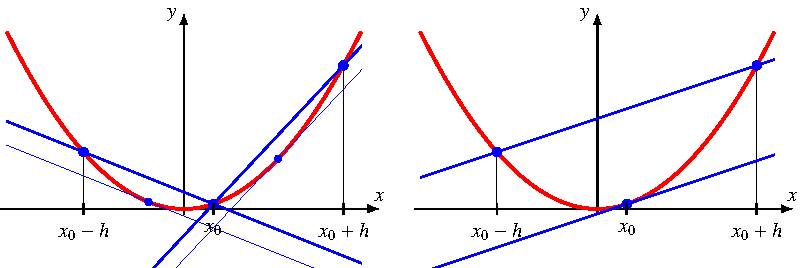
\includegraphics{chapters/70-pde/images/diffex.pdf}
\caption{Differenzenquotienten für die Funktion $f(x)=x^2$.
Die Vorwärts- und Rückwärtsdifferenzen im Punkt $x_0$ ergeben Approximationen
für die Ableitungen, die mit der wahren Ableitung im Punkt $x_0\pm \frac{h}2$
übereinstimmen.
Die symmetrische Differenz im Punkt $x_0$ ergibt genau die Steigung von $f(x)$
im Punkt $x_0$.
\label{buch:pde:diffex}}
\end{figure}
Um die Unterschiede zwischen den Fehlern der verschiedenen
Differenzapproximationen besser zu verstehen, approximieren wir die
Ableitungen der Funktion $f(x)=x^2$ im Punkt $x_0$ und bestimmen den
Fehler sowie den Punkt, in dem die Approximation den korrekten Ableitungswert
annimmt.
Die Vorwärts-, Rückwärts- und symmetrischen Differenzen sind
\begin{align*}
f'(x_0)
&\simeq
\frac{f(x_0+h)-f(x_0)}{h}
=
\frac{(x_0+h)^2-x_0^2}{h}
=
2x_0+h
&&=
f'(x_0 + {\textstyle\frac12}h)
\\
&\simeq
\frac{f(x_0)-f(x_0-h)}{h}
=
\frac{x_0+^2-(x_0-h)^2}{h}
=
2x_0-h
&&=
f'(x_0 - {\textstyle\frac12}h)
\\
&\simeq
\frac{f(x_0+h)-f(x_0-h)}{2h}
=
\frac{(x_0+h)^2-(x_0-h)^2}{2h}
=
\frac{4x_0h}{2h}=2x_0
&&=
f'(x_0).
\end{align*}
Für eine quadratische Funktion liefert also die symmetrische Differenz
den exakten Wert der Ableitung im Punkt $x_0$, während die Vorwärts-
und Rückwertsdifferenzen die Ableitungen in Punkten zwischen
den Gitterpunkten rechts bzw.~links von $x_0$
(Abbildung~\ref{buch:pde:diffex}).
\end{beispiel}

\subsubsection{Zweite Ableitungen}
\begin{figure}
\centering
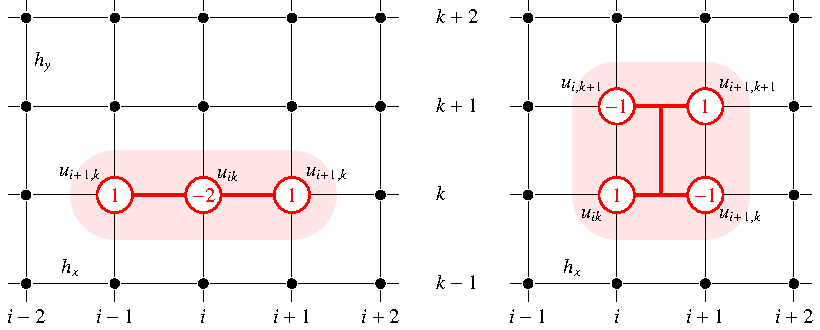
\includegraphics{chapters/70-pde/images/diff2.pdf}
\caption{Differenzenquotienten für die zweiten Ableitungen.
Links die zweite Ableitungen nach $x$, rechts die gemischte Ableitung.
In den roten Kreisen das Gewicht des zugehörigen Wertes der Funktion
im Differenzenquotienten.
\label{buch:pde:diff2}}
\end{figure}
Eine Approximation für die zweite Ableitung können wir erhalten als
Differenzenquotient aus der Vorwärts- und der Rückwärtsdifferenz:
\begin{align*}
\frac{\partial^2 u}{\partial x^2}(x_{ik})
&\simeq
\frac{1}{h_x}\biggl(
\frac{\partial u}{\partial x}(x_{i-\frac12,k})
-
\frac{\partial u}{\partial x}(x_{i+\frac12,k})
\biggr)
=
\frac{1}{h_x}
\cdot
\biggl(
\frac{u_{i+1,k}-u_{ik}}{h_x}
-
\frac{u_{ik}-u_{i-1,k}}{h_x}
\biggr)
\\
&=
\frac{u_{i+1,k}-2u_{ik}+u_{i-1,k}}{h_x^2}.
\end{align*}
Das Problem wird aber schwieriger, wenn eine gemischte Ableitung
approximiert werden soll.
Hier kann jede beliebige Kombination von Vorwärts- und Rückwärts-Differenzen
verwendet werden.
Mit Vorwärtsdifferenzen erhält man zum Beispiel
\begin{align*}
\frac{\partial^2u}{\partial x\,\partial y}(x_{ik})
&\simeq
\frac{1}{h_x}\biggl(
\frac{\partial u}{\partial y}(x_{i+1,k})
-
\frac{\partial u}{\partial y}(x_{ik})
\biggr)
\\
&=
\frac{1}{h_x}\biggl(
\frac{u_{i+1,k+1}-u_{i+1,k}}{h_y}
-
\frac{u_{i,k+1}-u_{ik}}{h_y}
\biggr)
\\
&=
\frac{1}{h_xh_y}(
u_{i+1,k+1}-u_{i+1,k}
-
u_{i,k+1}+u_{ik}
)
\end{align*}
Die in Abbildung~\ref{buch:pde:diff2} dargestellten ``Schablonen''
zeigen schematisch, wie die Ableitungen berechnet werden.
In den roten Kreisen um die beteiligten Knotenvariablen stehen die
Gewichte, mit denen die Knotenvariablen multipliziert werden müssen.

\subsubsection{Neumann-Randbedingungen}
Neumann-Randbedingungen geben die Ableitungen in Richtung der Normalen
auf dem Rand vor.
Die Diskretisation auf ein Gitter führt dazu, dass der Rand aus geraden
Teilstücken besteht, wo eine Normalenrichtung leicht zu definieren ist,
und Teilstücken, wo zusätzlicher Aufwand getrieben werden muss, überhaupt
die Richtung der Normalen zu definieren.
Für gerade Teilstücke des Randes können für die Approximation der
Normalableitung Vorwärts- oder Rückwärtsdifferenzen verwendet
werden.

\begin{beispiel}
\begin{figure}
\centering
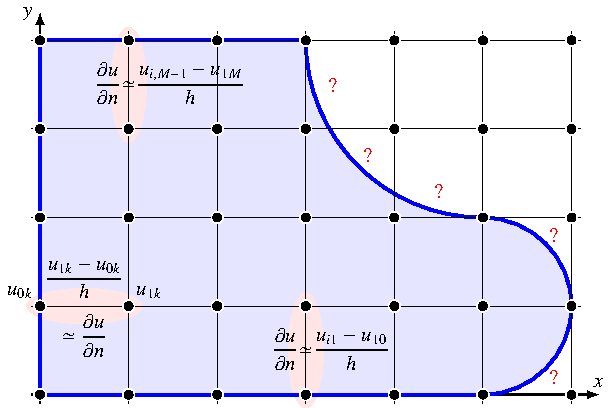
\includegraphics{chapters/70-pde/images/neumann.pdf}
\caption{Neumann-Randbedingungen sind in einem diskretisierten Gebiet 
einfach auszudrücken, solange die Gitterlinien mit dem Rand des 
Gebietes zusammenfallen.
Sie ergeben eine zusätzliche Gleichung zwischen den rot hinterlegten
Punkten.
Für die runden Teile des Randes gibt es keine einfachen Lösungen.
\label{buch:pde:neumann-analysis}}
\end{figure}
Zur Illustration des Vorgehens approximieren wir die Normalableitungen
für das Rechteckgebiet mit Rändern $x=0$, $x=Nh_x$, $y=0$ und $y=Mh_y$,
welches in Abbildung~\ref{buch:pde:neumann-analysis} dargestellt ist.
In Punkten $x_{0k}$ und $x_{Nk}$ auf den vertikalen Rändern
oder in Punkten $x_{i0}$ und $x_{iM}$ auf den horizontalen Rändern
können wir Vorwärts- bzw.~Rückwärtsdifferenzen verwenden:
\begin{align*}
\frac{\partial u}{\partial n}(x_{0k})
=
\frac{\partial u}{\partial x}(x_{0k})
&\simeq
\frac{u_{1k}-u_{0k}}{h_x}
&&\text{und}&
\frac{\partial u}{\partial n}(x_{Nk})
=
\frac{\partial u}{\partial x}(x_{Nk})
&\simeq
\frac{u_{Nk}-u_{N-1,k}}{h_x},
\\
\frac{\partial u}{\partial n}(x_{i0})
=
\frac{\partial u}{\partial y}(x_{i0})
&\simeq
\frac{u_{i1}-u_{i0}}{h_y}
&&\text{und}&
\frac{\partial u}{\partial n}(x_{iM})
=
\frac{\partial u}{\partial y}(x_{iM})
&\simeq
\frac{u_{iM}-u_{i,M-1}}{h_y}.
\end{align*}
Natürlich gelten die oben formulierten Vorbehalte bezüglich der
Zuverlässigkeit dieser Approximation, wir haben aber nicht die Möglichkeit,
symmetrische Differenzen zu verwenden, da keine Funktionswerte ausserhalb
des Gebietes bekannt sind.
\end{beispiel}


\subsubsection{Das Poisson-Problem}
\begin{figure}
\centering
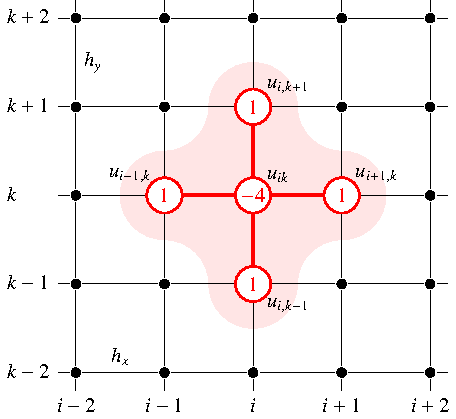
\includegraphics{chapters/70-pde/images/laplace.pdf}
\caption{Approximation des Laplace-Operators mit Summen von symmetrischen
Differenzen.
In den roten Kreisen die Gewichte, mit denen die Knotenvariablen 
multipliziert werden müssen, um den Ausdruck
\eqref{pde:eqn:poissongl} zu ergeben.
\label{buch:pde:laplace}}
\end{figure}
Das Poisson-Problem ist die Differentialgleichung
\begin{equation}
\frac{\partial^2 u}{\partial x^2}
+
\frac{\partial^2 u}{\partial y^2}
=
f
\label{buch:pde:poissondgl}
\end{equation}
auf einem Gebiet $\Omega$, wobei wir als Beispiel ein Quadrat
$\Omega = (0,1) \times (0,1)$ wählen.
Die abstrakte Theorie sagt, dass die Lösung der Differentialgleichung
eindeutig bestimmt ist, Randwerte $u(x)=g(x)$ für $x\in\partial\Omega$
vorgegeben werden.

\begin{figure}
\centering
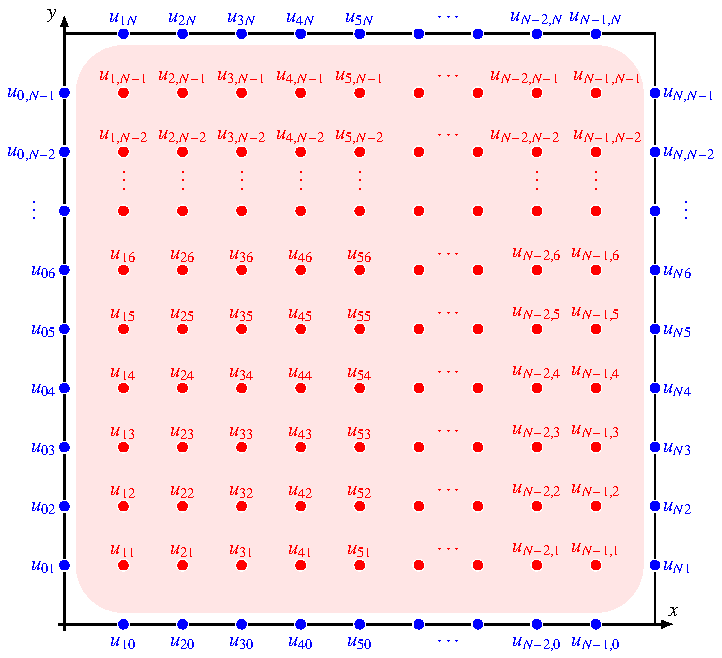
\includegraphics{chapters/70-pde/images/poisson.pdf}
\caption{Diskretisiertes Gebiet für die Differentialgleichung.
Die Werte in den blauen Punkten auf dem Rand sind durch die Randbedingungen
gegeben, nur die Werte in den roten Punkten müssen bestimmt werden.
\eqref{buch:pde:poissondgl}.
\label{buch:pde:poissongebiet}}
\end{figure}
Wir diskretisieren das Gebiet (Abbildung~\ref{buch:pde::poissongebiet})
mit Hilfe des Gitters mit Gitterkonstanten
$h=h_x=h_y=1/N$.
Wir erhalten die $(N+1)^2$ Unbekannten $u_{ik}$ mit $0\le i\le N$ und 
$0\le k\le N$.
Die Randbedingungen legen die Werte
\begin{align*}
u_{0k}&= g(0, kh)
&
u_{Nk}&= g(1, kh)
&&1\le k\le N
\\
u_{i0}&=g(ih,0)
&
u_{iN}&=g(ih,N)
&&
1\le i\le N
\end{align*}
fest.
$4N$ Unbekannte sind also bereits bestimmt, es bleiben noch
$(N+1)^2-4N = N^2-2N+1=(N-1)^2$ innere Werte zubestimmen.

Die Differentialgleichung kann für jeden Punkt im Inneren des Gebietes
$\Omega$ aufgestellt werden (die roten Punkte in
Abbildung~\ref{buch:pde:poissongebiet}), es gilt
\begin{align}
\frac{\partial^2 u}{\partial x^2}(u_{ik})
+
\frac{\partial^2 u}{\partial y^2}(u_{ik})
&=
\frac{u_{i+1,k}-2u_{ik}+u_{i-1,k}}{h^2}
+
\frac{u_{i,k+1}-2u_{ik}+u_{i,k-1}}{h^2}
\notag
\\
f_{ik}=f(x_{ik})
&=
\frac{1}{h^2} ( u_{i+1,k} + u_{i-1,k} + u_{i,k+1} + u_{i,k-1} - 4u_{ik}).
\label{pde:eqn:poissongl}
\end{align}
Alle diese $(N-1)^2$ Gleichungen sind linear.
Insbesondere haben wir gleich viele Gleichungen wie Unbekannte und 
dürfen daher davon ausgehen, dass, wie sich auch beweisen lässt, das
lineare Gleichungssystem
\eqref{pde:eqn:poissongl} 
für die verbleibenden Unbekannten regulär ist.
Die Diskretisation führt also die Lösung der partiellen Differentialgleichung
auf die Lösung eines linearen Gleichungssystems zurück.

%
% waermeleitung.tex -- Beispiel für Problemlösung mit finiten Differenzen
%
% (c) 2020 Prof Dr Andreas Müller, Hochschule Rapperswio
%
\subsection{Wärmeleitungsgleichung
\label{buch:subsection:waermeleitung}}
Als etwas ausführlicheres Beispiel soll in den folgenden Abschnitten
das Wärmeleitungsproblem auf einem Stab mit verschiedenen Randbedingungen
und Methoden zu lösen.
Dieser Abschnitt beginnt damit, das Problem und seine Diskretisierung
zu formulieren.
In den folgenden Abschnitten werden die Gleichungen dann für verschiedene
Randbedingungen numerisch gelöst.

\subsubsection{Die Wärmeleitungsgleichung}
Die Temperaturverteilung $u(x,t)$ auf einem Stab mit $x$-Koordinaten
zwischen $0$ und $1$ zur Zeit $t$ wird durch eine partielle
Differentialgleichung auf dem Gebiet
\[
\Omega = \{ (x,t)\;|\; 0 < x < 1\wedge 0<t\}
\]
beschrieben.
In der Wärmeleitungsgleichung
\begin{equation}
\frac{\partial u}{\partial t}
=
\kappa\frac{\partial^2 u}{\partial x^2}
\label{buch:pde:waerme:gleichung}
\end{equation}
ist die $\kappa$ eine Konstante, die Wärmeleitfähigkeit und
Wärmekapazität des Materials charaktersiert.

\subsubsection{Randbedingungen}
Zudem müssen Randbedingungen zur Zeit $t=0$ und an den Enden
des Stabes bei $x=0$ oder $x=1$ erfüllt sein.
Zur Zeit $t=0$ muss die initiale Temperaturverteilung $f(x)$ 
spezifiziert werden.

Dirichletrandbedingungen
\[
\begin{aligned}
u(x,0)&=f(x)&&x\in[0,1]
\\
u(x,t)=\frac{\partial u}{\partial x}(x,t)&=g(x)&&x\in \{0,1\}.
\end{aligned}
\]
am Rand des Intervals bedeuten, dass die Enden des Stabes mit Wärmereservoirs
verbunden sind, welche ihn auf einer vorgegebenen Temperatur halten.

Neumann-Randbedingungen
\[
\begin{aligned}
u(x,0)&=f(x)&&x\in[0,1]
\\
\frac{\partial u}{\partial n}(x,t)=\frac{\partial u}{\partial x}(x,t)&=g(x)&&x\in \{0,1\}.
\end{aligned}
\]
spezifizieren den Temperaturgradienten am Rande und legen damit fest,
wieviel Wärmeenergie in den Stab hineinfliesst oder ihn verlässt.
Im Falle $g(x)=0$ verschwindet der Gradient und Wärmefluss ist unterbunden.
Dies entspricht einem thermisch isolierten Stab.

\subsubsection{Energie}
Die physikalische Interpretation der
Gleichung~\ref{buch:pde:waerme:gleichung}
erlaubt, das Verhalten der Lösung abzuschätzen.
Dazu berechnen wir die Gesamtenergie
\[
U(t) = \int_0^1 u(x,t)\,dx,
\]
die im Intervall enthalten ist.
Die Wärmeleitungsgleichung~\ref{buch:pde:waerme:gleichung} erlaubt nun,
die Änderung der Energie mit der Zeit zu bestimmen.
Es gilt
\begin{align*}
\frac{dU(t)}{dt}
&=
\frac{d}{dt} \int_0^1 u(x,t)\,dx
=
\int_0^1 \frac{\partial u}{\partial t} (x,t)\,dx
=
\kappa \int_0^1 \frac{\partial^2u}{\partial x^2}(x,t)\,dx
=
\kappa \biggl[\frac{\partial u}{\partial x}\biggr]_0^1.
\end{align*}
Daraus lässt sich zum Beispiel ablesen, dass sich die Energie in
einem isolierten Stab, wo die Ableitungen an den Intervallenden
verschwinden, nicht ändert.
Oder dass Energie genau dann konstant bleibt, wenn die Steigung
in beiden Enden gleich gross ist, was gleichbedeutend ist damit,
dass der Wärmefluss durch beide Intervallenden gleich gross ist.

In allen Fällen kann man das Verhalten der Lösung für $t\to\infty$
bestimmen.
Dirichlet-Randbedingungen 
\[
u(0,t) = u_0 \qquad\text{und}\qquad u(1,t) = u_1
\]
sagen zum Beispiel, dass die beiden Enden des Stabes auf Temperatur
$u_0$ und $u_1$ gehalten werden.
Mit der Zeit wird sich eine stationäre Temperaturverteilung, also eine
Temperaturverteilung, die sich mit der Zeit nicht mehr ändert.
Eine solche hat zweite Ableitung
\[
\frac{\partial^2u}{\partial x^2}
=
\frac{1}{\kappa} \frac{\partial u}{\partial t} = 0.
\]
Die Funktion $x\mapsto u(x,t)$ muss also linear sein, was auf die
stationäre Temperaturverteilung
\[
u_\infty(x) = tu_1 + (1-t)u_0
\]
führt.

Für konstante Neumann-Randbedingungen
\[
\frac{\partial u}{\partial t}(0) = v_0
\qquad\text{und}\qquad
\frac{\partial u}{\partial t}(1) = v_1
\]
ist der Wärmefluss in den Stab konstant, es gilt
\[
\frac{dU(t)}{dt} = (v_1-v_0)t + U(0).
\]
Insbesondere kann man nicht erwarten, dass es eine stationäre Lösung
gibt.
Vielmehr erwartet man eine Lösung, die linear mit der Zeit anwächst.
Eine lineare Funktion von $x$ kann nicht funktionieren, weil diese
auf gleichen Wärmefluss durch die beiden Intervallenden führen würde.
Wir versuchen daher den quadratischen Ausdruck.
\[
u_s(x,t) = ax^2 + bx + c + dt.
\]
Tatsächlich sind die Ableitungen
\begin{align*}
\frac{\partial u_s}{\partial t}
&=
d
\\
\frac{\partial^2 u_s}{\partial x^2}
&=
2a.
\end{align*}
Eingesetzt in die Differentialgleichung finden wir den Wert von $a$
\begin{equation*}
d=2a\kappa
\end{equation*}
Um die Werte von $a$ und $b$ zu bestimmen, müssen wir die Randbedingungen
bemühen:
\begin{align*}
v_0=\frac{\partial u}{\partial x}(0) &= b &&\Rightarrow& b &= v_0
\\
v_1=\frac{\partial u}{\partial x}(1) &= 2a + b &&\Rightarrow& a &= \frac{v_1-v_0}2
\end{align*}
Damit ist auch $d=\kappa (v_1-v_0)$ bestimmt.
Einzig $c$ lässt sich auf diesem Weg nicht bestimmen, dazu sind weitere
Dirichlet-Randbedingungen erfoderlich.

\subsubsection{Diskretisation}
Zur Diskretisation verwenden wir ein Gitter mit Gitterkonstanten
$h_x=1/N$ und $h_t$.
Die zu bestimmenden Unbekannten sind die $u_{ik}$ mit
$0\le i\le N$ und $k\ge 0$.
Die Randbedingungen auf dem Rand $t=0$ geben die Werte 
\[
u_{i0} = u(ih_x,0) = f(ih_x) =: f_i
\]
vor.

Für Dirichlet-Randbedingungen an den Intervallenden legen die Werte von
$u_{ik}$ für $i=0$ und $i=N$ fest.
Die Variablen $u_{0k}$ und $u_{Nk}$ sind also nicht Unbekannte sondern
vorgegebene Werte.

Die Neumann-Randbedingungen am linken und rechten Rand können mit Hilfe
der Vorwärts- bzw.~Rückwärts-Differenzen approximiert werden:
\begin{align*}
\frac{\partial u}{\partial n}(x_{0k})
&\simeq
\frac{u_{1k}-u_{0k}}{h_x}
=
0
&&\text{und}&
\frac{\partial u}{\partial n}(x_{0k})
&\simeq
\frac{u_{Nk}-u_{N-1,k}}{h_x}
=
0
\intertext{Dies bedeutet, dass die beiden Werte nahe des Randes
gleich sind}
u_{0k}&=u_{1k}&&\text{und}&u_{Nk}&=u_{N-1,k}.
\end{align*}
Die Differentialgleichung verwendet die zweite Ableitung nach $x$, 
für die wir die Approximation
\[
\frac{\partial^2u}{\partial x^2}(x_{ik})
=
\frac{u_{i+1,k}-2u_{ik}+u_{i-1,k}}{h_x^2}
\]
verwenden können.

\subsubsection{Matrixform}
Da die Werte $u(x,0)=f(x)$ von $u$ zur Zeit $t=0$ bereits bekannt
sind, wird die numerische Lösung nacheinander die Variablen
$u_{ik}$ mit $k=1,2,3,\dots$ bestimmen.
Der Schritt $k\to k+1$ kann etwas kompakter beschrieben und vor allem
leichter analysiert werden, wenn wir die Werte $u_{ik}$ für gegebenes $k$
in den Vektor
\[
u_k = \begin{pmatrix}
u_{0k}\\
u_{1k}\\
\vdots\\
u_{ik}\\
\vdots\\
u_{Nk}
\end{pmatrix}
\]
zusammenfassen.
Für homogene Randbedingungen ist der Zusammnenhang zwischen $u_k$
und $u_{k+1}$ eine lineare Funktion, es muss also eine Matrix geben,
welche $u_{k+1}=Au_k$.

Sind die Randbedingungen nicht homogen, kann man nicht mehr unbeding
eine Zeitunabhängige Matrix $A$ finden, vielmehr kann die Matrix
in jedem Zeitschritt verschieden sein.
Ausserdem kann in jedem Zeitschritt ein konstanter Wert hinzukommen.
Insgesamt gibt es also eine Matrix $A_k$ und ein Vektor $b_k$ derart,
dass $u_{k+1} = A_ku_k + b_k$.


Für die erste Ableitung nach der Zeit könnten Vorwärts- oder
Rückwärts-Differenzen verwendet werden, in beiden Fällen entsteht
ein unvermeidbarer Fehler und ein jeweils anderes numerisches
Lösungsverfahren.

\subsubsection{Euler-Verfahren}
\begin{figure}
\centering
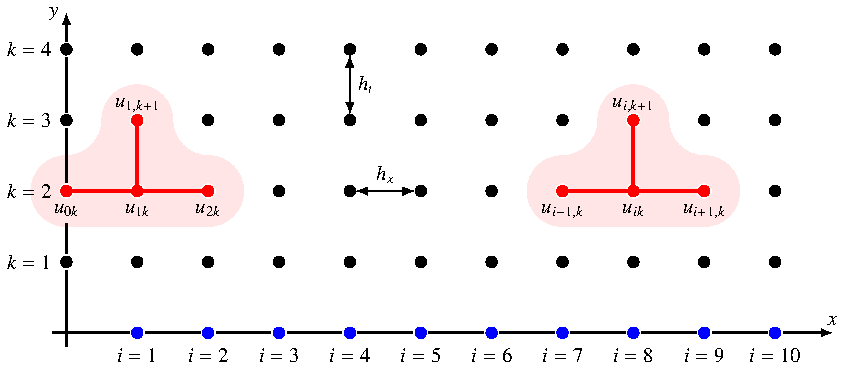
\includegraphics{chapters/70-pde/images/euler.pdf}
\caption{Euler-Verfahren für das Wärmeleitungsproblem.
\label{buch:pde:figure:euler}}
\end{figure}
Wir müssen jetzt die Differentialgleichung des Wärmelitungsproblems
diskretisieren.
Für die zweite Ableitung verwenden wir zweite Differenzen
Für die ersten Ableitungen haben wir verschiedene Optionen, wir
verwenden Vorwärtsdifferenzen, also
\begin{align}
\frac{\partial u}{\partial x}(x_{ik})
\simeq
\frac{u_{i,k+1}-u_{ik}}{h_t}
&=
\kappa
\frac{\partial^2u}{\partial x^2}(x_{ik})
\simeq
\kappa
\frac{u_{i,k-1}-2u_{ik}+u_{i,k+1}}{h_x^2}
\notag
\\
u_{i,k+1}
&=
u_{ik} + \frac{h_t\kappa}{h_x^2} (u_{i-1,k}-2u_{ik}+u_{i+1,k})
\label{buch:pde:waerme:euler}
\end{align}
für die inneren Punkte.
In Matrixform kann dies als
\[
\begin{pmatrix}
\vdots\\
u_{i,k+1}\\
\vdots
\end{pmatrix}
=
\begin{pmatrix}
&&&&\\
0&\dots
	&\displaystyle\frac{h_t\kappa}{h_x^2}
		&\displaystyle1-\frac{2h_t\kappa}{h_x^2}
			&\displaystyle\frac{h_t\kappa}{h_x^2}
				&\dots
					&0\\
&&&&
\end{pmatrix}
\begin{pmatrix}
\vdots\\
u_{i-1,k}\\
u_{ik}\\
u_{i+1,k}\\
\vdots
\end{pmatrix}
\]
geschrieben werden.
Wir kürzen den gemeinsamen Faktor $c=h_t\kappa/h_x^2$ ab und erhalten
die Form
\[
u_{k+1}
=
\begin{pmatrix}
\ddots&\ddots&\ddots&    &      &      &      \\
      &     c&  1-2c&  c &      &      &      \\
      &      &    c &1-2c&  c   &      &      \\
      &      &      &  c &1-2c  &  c   &      \\
      &      &      &    &\ddots&\ddots&\ddots
\end{pmatrix}
u_k.
\]
Die Lösung wird sich durch Iteration dieser Matrix finden lassen,
Konvergenz wird allein von $c$ abhängen.
Wir erwarten also, ein Konvergenz-Kriterium basierend auf $c$.

Die Gleichung~\eqref{buch:pde:waerme:euler} gilt nur für innere Punkte.
Für die Variablen $u_{0k}$, $u_{1k}$, $u_{N-1,k}$ und $u_{Nk}$ müssen
wir aus den Randbedingungen zusätzliche Gleichungen für die Randwerte
ableiten müssen.

\subsubsection{Rückwärts-Verfahren}
\begin{figure}
\centering
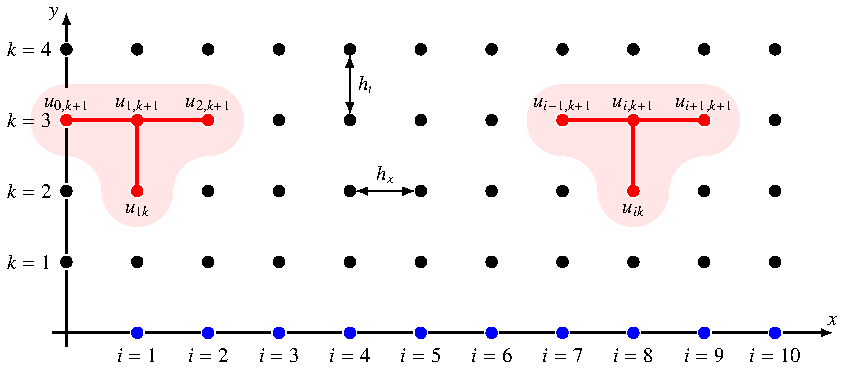
\includegraphics{chapters/70-pde/images/rueckwaerts.pdf}
\caption{Verwendung von Rückwärts-Differenzen für die Wärmeleitungsgleichung
\label{buch:pde:figure:rueckwaerts}}
\end{figure}
Statt der Vorwärts-Differenz kann man auch die Rückwärts-Differenz für
die erste Ableitung nach der Zeit verwenden.
Die diskretisierte Gleichung wird dann
\begin{align*}
\frac{u_{ik}-u_{i,k-1}}{h_t}
\simeq
\frac{\partial u}{\partial x}(x_{ik})
&=
\kappa\frac{\partial^2 u}{\partial x^2}(x_{ik})
\simeq
\frac{u_{i-1,k}-2u_{ik} + u_{i+1,k}}{h_x}.
\\
-cu_{i-1,k}
+
(1+2c)u_{ik}
-cu_{i+1,k}
&=u_{i,k-1}.
\end{align*}
In Matrixform kann man dies als
\[
\begin{pmatrix}
%\ddots&\ddots&\ddots&    &      &      &      \\
      &    -c&  1+2c& -c &      &      &      \\
      &      &   -c &1+2c& -c   &      &      \\
      &      &      & -c &1+2c  & -c   &      \\
      &      &      &    &\ddots&\ddots&\ddots
\end{pmatrix}
u_k
=
u_{k-1}
\]
schreiben.
Wieder gelten diese Gleichungen nur für innere Punkte.
Abbildung~\ref{buch:pde:figure:rueckwarts} zeigt, wie die Gleichungen
die Knotenwerte untereinander verknüpfen.

\subsubsection{Crank-Nicholson-Verfahren}
\begin{figure}
\centering
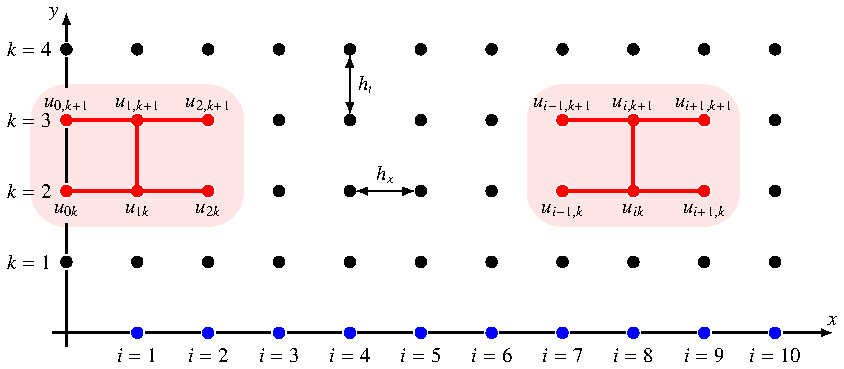
\includegraphics{chapters/70-pde/images/cngrid.pdf}
\caption{Verwendung der Knotenvariablen im Crank-Nicholson-Verfahren.
\label{buch:pde:figure:cngrid}}
\end{figure}
Sowohl Vorwärts- wie auch Rückwärts-Differenzen bestimmen die erste
Ableitung nach der Zeit eigentlich für einen Zeitpunkt zwischen 
den Vielfachen von $h_t$.
Für diese Zeitpunkte stehen aber keine Funktionswerte zur Verfügung, 
um damit die Gleichung aufzustellen.
Das Crank-Nicholson-Verfahren schlägt daher vor, den Mittelwert der
zweiten Ableitungen zu benachbarten Zeitpunkten als Wert für den
Zwischenzeitpunkt zu verwenden.
Damit wird die Wärmeleitungsgleichung approximiert durch
\begin{align*}
\frac{u_{i,k+1}-u_{ik}}{h_t}
\simeq
\frac{\partial u}{\partial x}(x_{ik})
&=
\kappa
\frac{\partial^2 u}{\partial x^2}(x_{ik})
\simeq
\frac{\kappa}2\biggl(
\frac{u_{i-1,k+1}-2u_{i,k+1}+u_{i+1,k+1}}{h_x^2}
+
\frac{u_{i-1,k}-2u_{i,k}+u_{i+1,k}}{h_x^2}
\biggr)
\\
2u_{i,k+1}-2u_{ik}
&=
c(
u_{i-1,k+1}-2u_{i,k+1}+u_{i+1,k+1}
+
u_{i-1,k}-2u_{i,k}+u_{i+1,k}
)
\end{align*}
Verschiebt man die Terme nach Zeitpunkt auf die beiden Seiten
der Gleichung erhält man
\begin{equation}
-cu_{i-1,k+1}+2(1+c)u_{i,k+1}-cu_{i+1,k+1}
=
cu_{i-1,k}+2(1-c)u_{i,k}+cu_{i+1,k},
\end{equation}
was sich leichter in Matrixform 
\begin{equation}
\begin{pmatrix}
&\ddots& \ddots &        &        &        &        \\
&  -c  & 2(1+c) &  -c    &        &        &        \\
&      &  -c    & 2(1+c) &  -c    &        &        \\
&      &        &  -c    & 2(1+c) &  -c    &        \\
&      &        &        & \ddots & \ddots &        
\end{pmatrix}
u_{k+1}
=
\begin{pmatrix}
&\ddots&\ddots  &        &        &        &        \\
&   c  & 2(1-c) &   c    &        &        &        \\
&      &   c    & 2(1-c) &   c    &        &        \\
&      &        &   c    & 2(1-c) &   c    &        \\
&      &        &        &\ddots  & \ddots &        
\end{pmatrix}
u_k
\end{equation}
bringen lässt.

\subsection{Wärmeleitungsgleichung mit Dirichlet-Randbedingungen
\label{buch:pde:subsection:waerme:dirichlet}}
Die bisher formulierten Gleichungen berücksichtigen die
Randbedingungen nicht.
Dirichlet-Rand\-bedingungen am linken und rechten Rand des Intervalls
legen die Werte $u_{0k}$ und $u_{Nk}$ fest.
Wir möchten dies wieder in Matrixform schreiben.
Da die Randbedingungen nicht von $u$ abhängen, muss dies in der Form
$u_{k+1}=Au_k + b_k$ möglich sein, was nur geht, wenn
\begin{equation}
u_{k+1}
=
\underbrace{
\begin{pmatrix}
 0  &   0  &  0   &      &      &      &      &      &      \\
 c  & 1-2c &  c   &      &      &      &      &      &      \\
    &  c   & 1-2c &  c   &      &      &      &      &      \\
    &      &\ddots&\ddots&\ddots&      &      &      &      \\
    &      &      &  c   & 1-2c &  c   &      &      &      \\
    &      &      &      &\ddots&\ddots&\ddots&      &      \\
    &      &      &      &      &  c   & 1-2c &  c   &      \\
    &      &      &      &      &      &  c   & 1-2c &  c   \\
    &      &      &      &      &      &  0   &  0   &  0   
\end{pmatrix}}_{\displaystyle A\mathstrut}
u_k
+
\underbrace{
\begin{pmatrix}
g_{0k}\\
0     \\
0     \\
\vdots\\
0     \\
\vdots\\
0     \\
0     \\
g_{Nk}
\end{pmatrix}}_{\displaystyle b_k\mathstrut}
\end{equation}
für die Randwerte $g$.

Für homogene Randbedingungen wird die Situation etwas einfacher zu
analysieren, denn dann ist $b_k=0$.
Wir erwarten, dass die Lösung exponentiell gegen $0$ konvergiert,
das System ``kühlt aus''.
Da die Randbedingungen $u_{0k}=u_{Nk}=0$ erzwingen, kann man diese 
Variablen weglassen die Vektoren $u$ und die Matrix $A$ verkürzen auf
\begin{equation}
\tilde{u}_{k+1}
=
\begin{pmatrix}
u_{1,k+1}\\
u_{2,k+1}\\
\vdots\\
u_{i,k+1}\\
\vdots\\
u_{N-1,k+1}\\
u_{N,k+1}
\end{pmatrix}
=
\underbrace{
\begin{pmatrix}
 1-2c &  c   &      &      &      &      &      \\
  c   & 1-2c &  c   &      &      &      &      \\
      &\ddots&\ddots&\ddots&      &      &      \\
      &      &  c   & 1-2c &  c   &      &      \\
      &      &      &\ddots&\ddots&\ddots&      \\
      &      &      &      &  c   & 1-2c &  c   \\
      &      &      &      &      &  c   & 1-2c \\
\end{pmatrix}}_{\displaystyle \tilde{A}\mathstrut}
\begin{pmatrix}
u_{1k}\\
u_{2k}\\
\vdots\\
u_{ik}\\
\vdots\\
u_{N-1,k}\\
u_{Nk}
\end{pmatrix}
=
A
\tilde{u}_k
\end{equation}
Die Lösung $u$ entsteht also durch Iteration mit der Matrix $\tilde{A}$.
Der Spektralradius der Matrix gibt Auskunft darüber, ob das Verfahren
konvergiert.
Da die Matrix $\tilde{A}$ symmetrisch ist, sind alle Eigenwerte reell.
\begin{figure}
\centering
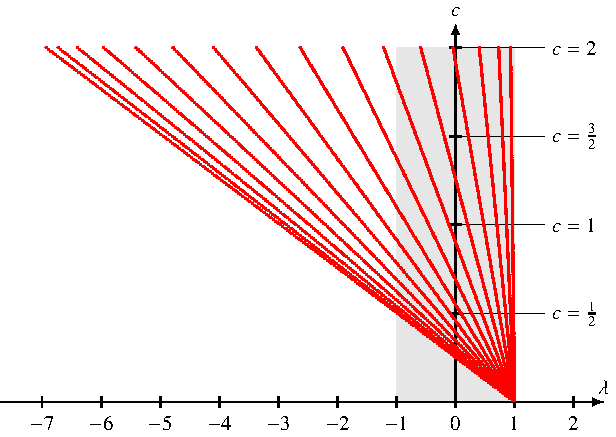
\includegraphics{chapters/70-pde/images/explizitspektrum.pdf}
\caption{Spektrum der Matrix $\tilde{A}$ für $N=16$,
die sich für das Euler-Verfahren mit
homogenen Dirichlet-Randwerte ergibt.
Nur für $c<2$ ist der Spektralradius $<1$.
\label{buch:pde:waerme:explizitspektrum}}
\end{figure}
In Abbildung~\ref{buch:pde:waerme:explizitspektrum} sind die Eigenwerte
von $\tilde{A}$ dargestellt.
Man kann erkennen, dass nur für $c<\frac12$ der Spektralradius $<1$
wird.
Daraus ergibt sich das Kriterium
\[
\frac{2\kappa h_t}{h_x^2} < 1
\]
für die Konvergenz des Verfahrens.

Für das Rückwärtsverfahren sieht die Matrix etwas anders aus, es gilt
\begin{equation}
\begin{pmatrix}
   0  &    0  &   0  &      &      &      &      &      &      \\
  -c  &  1+2c &  -c  &      &      &      &      &      &      \\
      &   -c  & 1+2c &  -c  &      &      &      &      &      \\
      &       &\ddots&\ddots&\ddots&      &      &      &      \\
      &       &      &  -c  & 1+2c &  -c  &      &      &      \\
      &       &      &      &\ddots&\ddots&\ddots&      &      \\
      &       &      &      &      &  -c  & 1+2c &  -c  &      \\
      &       &      &      &      &      &  -c  & 1+2c &  -c  \\
      &       &      &      &      &      &   0  &   0  &   0  
\end{pmatrix}
u_{k+1}
=
Bu_{k+1}
=
u_k + b_k
\end{equation}
Für den Fall homogener Randbedingungen werden auch hier wieder
nur die ``inneren'' Koeffizienten
\[
\tilde{B}
=
\begin{pmatrix}
 1+2c &  -c  &      &      &      &      &      \\
  -c  & 1+2c &  -c  &      &      &      &      \\
      &\ddots&\ddots&\ddots&      &      &      \\
      &      &  -c  & 1+2c &  -c  &      &      \\
      &      &      &\ddots&\ddots&\ddots&      \\
      &      &      &      &  -c  & 1+2c &  -c  \\
      &      &      &      &      &  -c  & 1+2c 
\end{pmatrix}
\]
der Matrix $B$ nötig.
Die Lösung findet man dann aus $\tilde{B}\tilde{u}_{k+1}=\tilde{u}_k$
durch Iteration $\tilde{u}_{k+1}=\tilde{B}^{-1} \tilde{u}_k$.
Konvergenz wird wieder bestimmt durch den Spektralradius $\varrho{\tilde{B}}$,
der, wie Abbildung~\ref{buch:pde:waerme:implizitspektrum} zeigt, immer
$<1$ ist.
Das Rückwärtsverfahren ist also immer konvergent, ganz unabhängig von
den relativen Schrittweiten.
\begin{figure}
\centering
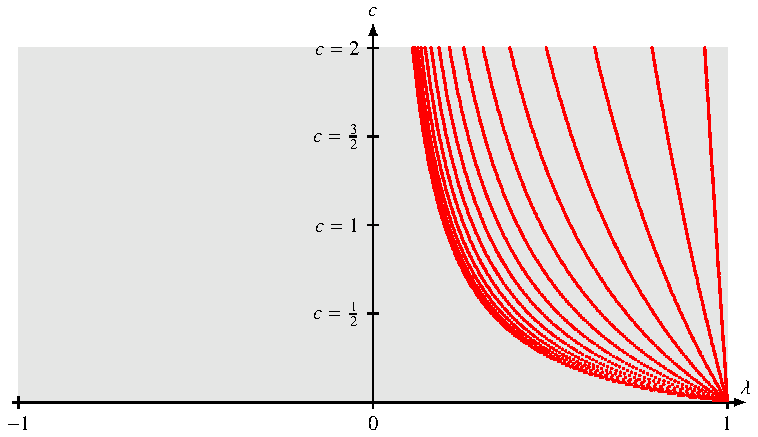
\includegraphics{chapters/70-pde/images/implizitspektrum.pdf}
\caption{Eigenwertspektrum der Matrix $\tilde{B}^{-1}$ für das 
Rückwärts-Verfahren.
Der Spektralradius ist unabhängig von $c$ immer $<1$.
\label{buch:pde:waerme:implizitspektrum}}
\end{figure}

Für das Crank-Nicholson-Verfahren ist, welches wir hier nur für homogene
Randbedingungen betrachten wollen.
Aus der Gleichung
\begin{gather*}
\tilde{C}u_{k+1}
=
\begin{pmatrix}
2(1+c)&  -c  &      &      &      &      &      \\
   -c &2(1+c)&  -c  &      &      &      &      \\
      &   -c &2(1+c)&  -c  &      &      &      \\
      &      &\ddots&\ddots&\ddots&      &      \\
      &      &      &\ddots&\ddots&\ddots&      \\
      &      &      &      &   -c &2(1+c)&  -c  \\
      &      &      &      &      &  -c  &2(1+c)
\end{pmatrix}
u_{k+1}
\qquad
\qquad
\qquad
\\
\qquad
\qquad
\qquad
=
\tilde{D}u_{k}
=
\begin{pmatrix}
2(1-c)&   c  &      &      &      &      &      \\
    c &2(1-c)&   c  &      &      &      &      \\
      &    c &2(1-c)&   c  &      &      &      \\
      &      &\ddots&\ddots&\ddots&      &      \\
      &      &      &\ddots&\ddots&\ddots&      \\
      &      &      &      &    c &2(1-c)&   c  \\
      &      &      &      &      &   c  &2(1-c)
\end{pmatrix}
u_k
\end{gather*}
folgern wir, dass die Iteration $u_{k+1} = \tilde{C}^{-1}\tilde{D} u_k$
die Lösung der Gleichung liefert.
\begin{figure}
\centering
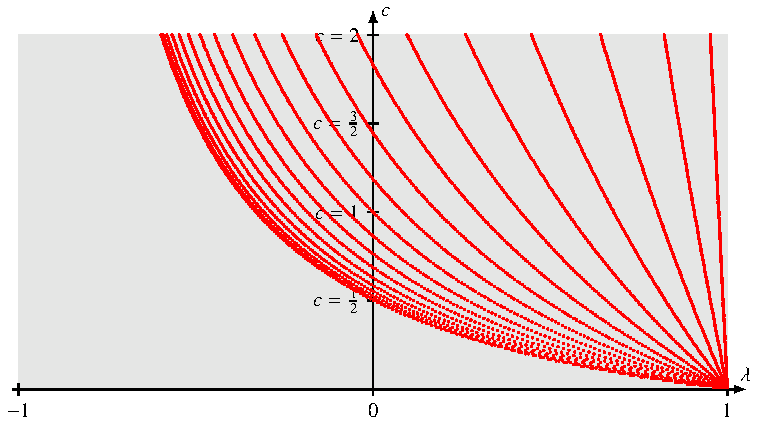
\includegraphics{chapters/70-pde/images/cnspektrum.pdf}
\caption{Eigenwertspektrum für das Crank-Nicholson-Verfahren
\label{buch:pde:waerme:cnspektrum}}
\end{figure}
Das Spektrum von $\tilde{C}^{-1}\tilde{D}$ ist in
Abbildung~\ref{buch:pde:waerme:cnspektrum} dargestellt und zeigt,
dass auch das Crank-Nicholson-Verfahren immer konvergiert unabhängig von
der Schrittweite $h_t$.

\subsection{Wärmeleitungsgleichung mit Neumann-Randbedingungen
\label{buch:pde:subsection:waerme:neumann}}
Die Neumann-Randbedingungen legen nicht Werte in den Randpunkten fest,
sondern liefern nur Gleichungen zwischen den Variablen nahe dem Rand.
Sie ändern damit die Koeffizientenmatrix des Gleichungssystems und haben
nicht nur Einfluss auf konstante Vektoren $b_k$ wie in
Abschnitt~\ref{buch:pde:subsection:waerme:dirichlet}.

\subsubsection{Neumann-Randbedingungen}
Wir betrachten in diesem Abschnitt nur homogene Neumann-Randbedingungen.
Die Randbedingung am linken und rechten Rand verlangt, dass $u_{0k}=u_{1k}$
und $u_{N-1,k}=u_{Nk}$ gelten muss.
Dies bedeutet, dass die Randwerte $u_{0k}$ und $u_{Nk}$ mit der
gleichen Formel berechnet werden können wie die Werte für $u_{1k}$ und
$u_{N-1,k}$.
Wir können damit die Variablen $u_{0k}$ und $u_{Nk}$ aus allen
Gleichungen eliminieren, indem wir sie durch $u_{1k}$ und $u_{N-1,k}$ 
ersetzen.

\subsubsection{Euler-Verfahren}
Aus den Gleichungen
\begin{align*}
u_{1,k+1} &= c u_{0k} + (1-2c) u_{1k} + c u_{2k} \\
u_{N-1,k+1} &= c u_{N-2,k} + (1-2c) u_{N-1,k} + c u_{Nk} 
\end{align*}
am Rand des Gebietes werden nach den Ersetzungen
$u_{0k}\to u_{1k}$
und
$u_{Nk}\to u_{N-1,k}$
die Gleichungen
\begin{align*}
u_{1,k+1}
&=
(1-c) u_{1k} + c u_{2k}
\\
u_{N-1,k+1}
&=
c u_{N-2,k} + (1-c) u_{N-1,k}.
\end{align*}
Die Matrix des Euler-Verfahrens wird damit zu
\begin{equation}
\tilde{u}_{k+1}
=
\underbrace{
\begin{pmatrix}
 1- c &  c   &      &      &      &      &      \\
  c   & 1-2c &  c   &      &      &      &      \\
      &\ddots&\ddots&\ddots&      &      &      \\
      &      &  c   & 1-2c &  c   &      &      \\
      &      &      &\ddots&\ddots&\ddots&      \\
      &      &      &      &  c   & 1-2c &  c   \\
      &      &      &      &      &  c   & 1- c 
\end{pmatrix}}_{\displaystyle A}
\tilde{u}_k.
\end{equation}
Die Konvergenz des Verfahrens hängt wieder vom Spektralradius ab.
Diesmal können wir aber nicht erwarten, dass alle Eigenwerte
Betrag $<1$ haben werden.
Die Zeilen- und Spaltensumme der Matrix $A$ ist immer $1$, d.~h.~die
ein konstanter Vektor wird auf sich selbst abgebildet.
Insbesondere gibt es einen Eigenvektor zum Eigenwert $1$,
der Spektralradius kann also nicht kleiner als $1$ sein. 
\begin{figure}
\centering
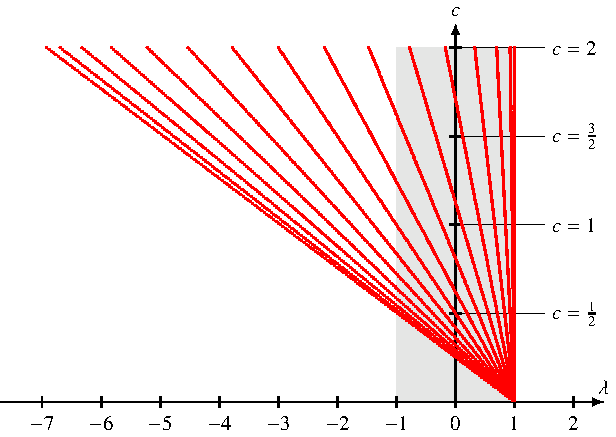
\includegraphics{chapters/70-pde/images/explizitneumann.pdf}
\caption{Eigenwertspektrum des Euler-Verfahrens für
Neumann-Randbedingungen.
Der Eigenwert $1$ ist einfach,
für $c<\frac12$ ist der Spektralradius $1$.
\label{buch:pde:waerme:explizit:neumannspektrum}}
\end{figure}
Für $c<1$ konvergiert das Verfahren daher gegen die konstante
Temperaturverteilung.
\begin{figure}
\centering
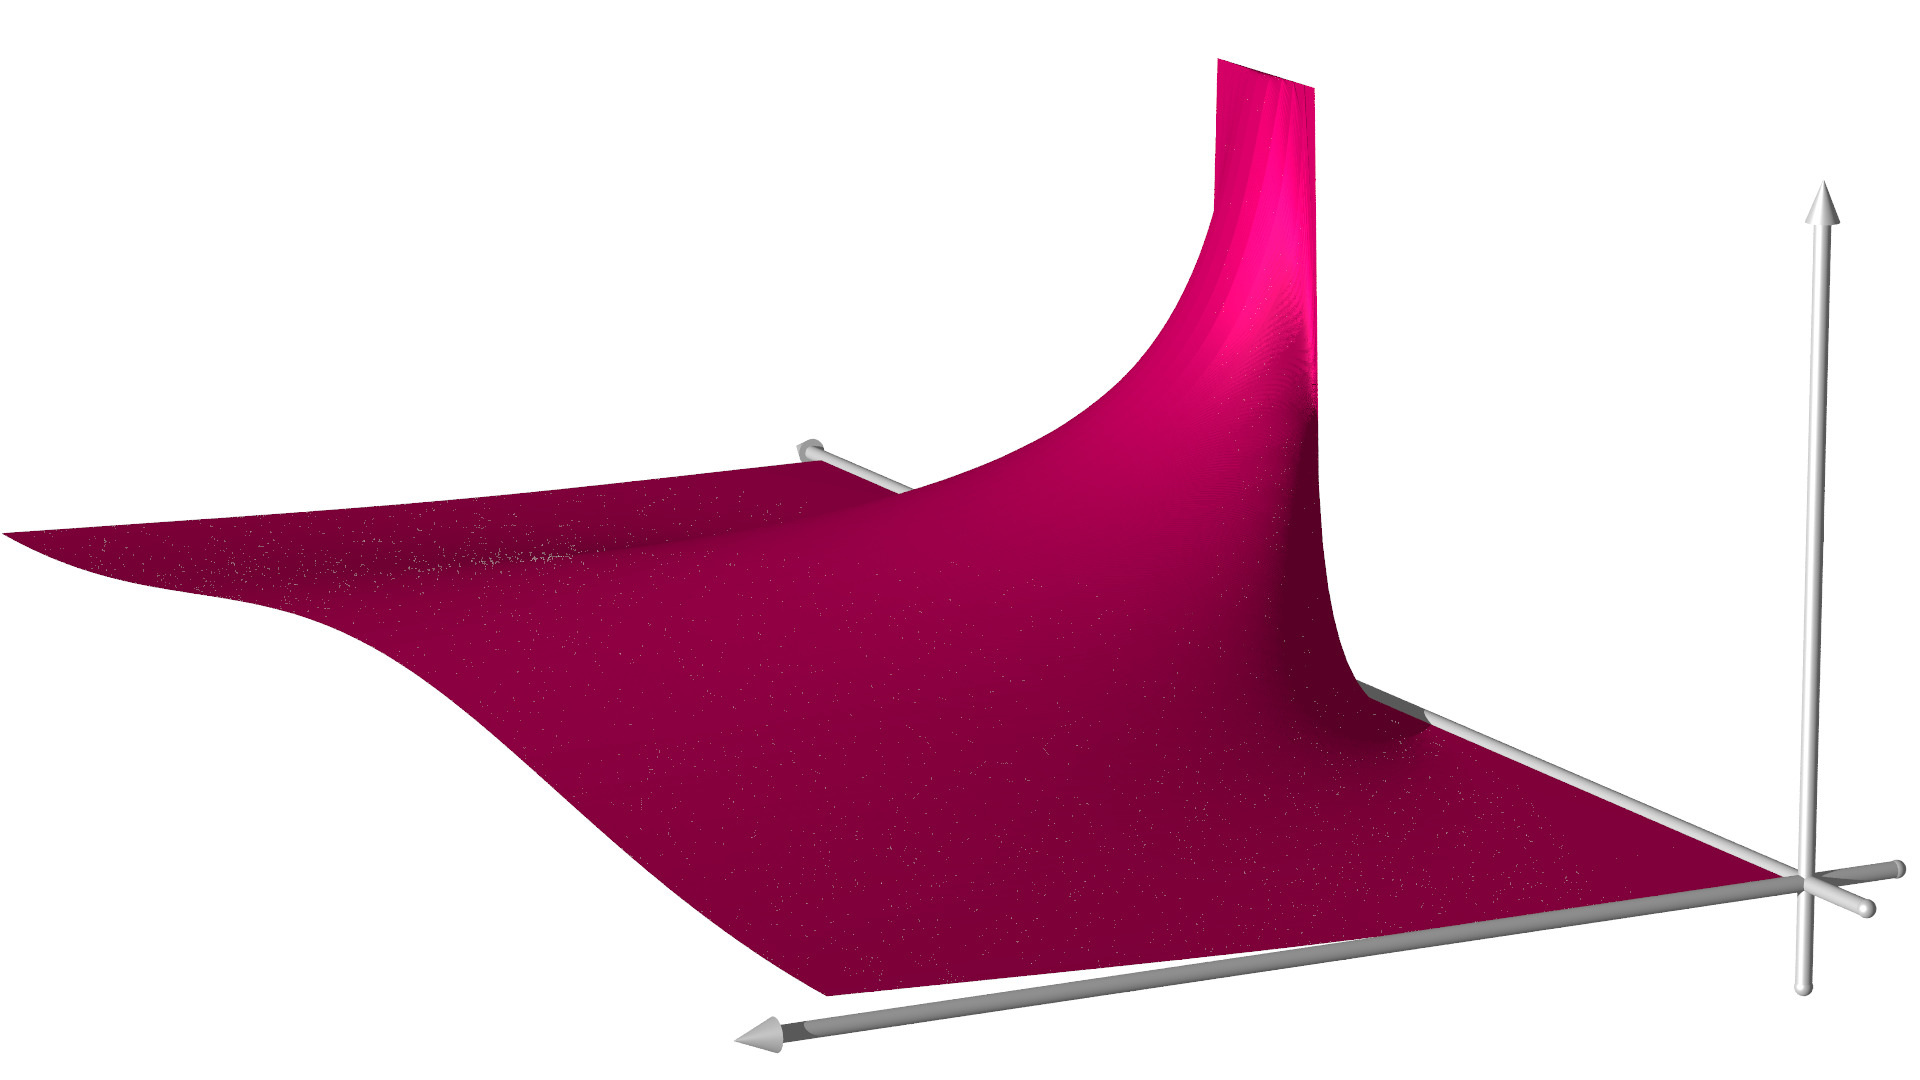
\includegraphics[width=\hsize]{chapters/70-pde/images/explizit.jpg}
\caption{Lösung der Wärmeleitungsgleichung mit dem Euler-Verfahren.
\label{buch:pde:waerme:figure:euler}}
\end{figure}
Die numerische Durchführung des Verfahrens mit geeigneten Werten von
$h_x$ und $h_t$ derart, dass $c<\frac12$ ist, führt auf die
Lösungsfläche in Abbildung~\ref{buch:pde:waerme:figure:euler}.

\subsubsection{Rückwärtsverfahren}
Auch für das Rückwärtsverfahren können wir für Neumann-Randbedinungen
die Matrixgleichung
\begin{equation}
Bu_k
=
\begin{pmatrix}
 1+c & -c   &      &      &      &      &      &     \\
 -c  & 1+2c & -c   &      &      &      &      &     \\
     &  -c  & 1+2c & -c   &      &      &      &     \\
     &      &\ddots&\ddots&\ddots&      &      &     \\
     &      &      &\ddots&\ddots&\ddots&      &     \\
     &      &      &      &  -c  & 1+2c & -c   &     \\
     &      &      &      &      &  -c  & 1+2c & -c  \\
     &      &      &      &      &      &  -c  & 1+c 
\end{pmatrix}
u_k
=
u_{k-1}
\end{equation}
finden.
Auch diese Matrix hat den konstanten Vektor als einzigen Eigenvektor
zum Eigenwert $1$.
Wie bei Dirichlet-Randbedingungen ist das Spektrum, dargestellt in
Abbildung~\ref{buch:pde:waerme:implizit:neumannspektrum}, bis auf den
einen Eigenwert $1$ im Intervall $(0,1)$ enthalten, so dass das
Verfahren konvergiert.
Die Lösung ist dargestellt in
Abbildung~\ref{buch:pde:waerme:figure:rueckwaerts}.
\begin{figure}
\centering
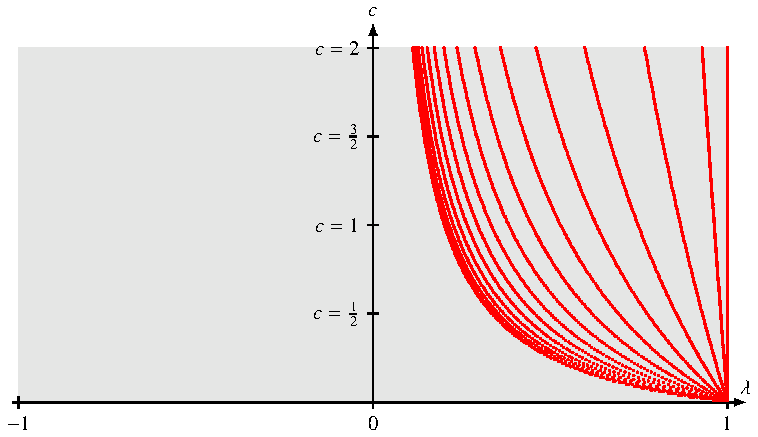
\includegraphics{chapters/70-pde/images/implizitneumann.pdf}
\caption{Das Eigenwertspektrum für das Rückwärtsverfahren für
Neumann-Randbedingungen enthält eine einzelnen Eigenwert $1$, alle
anderen Eigenwerte haben Betrag $<1$.
\label{buch:pde:waerme:implizit:neumannspektrum}}
\end{figure}
\begin{figure}
\centering
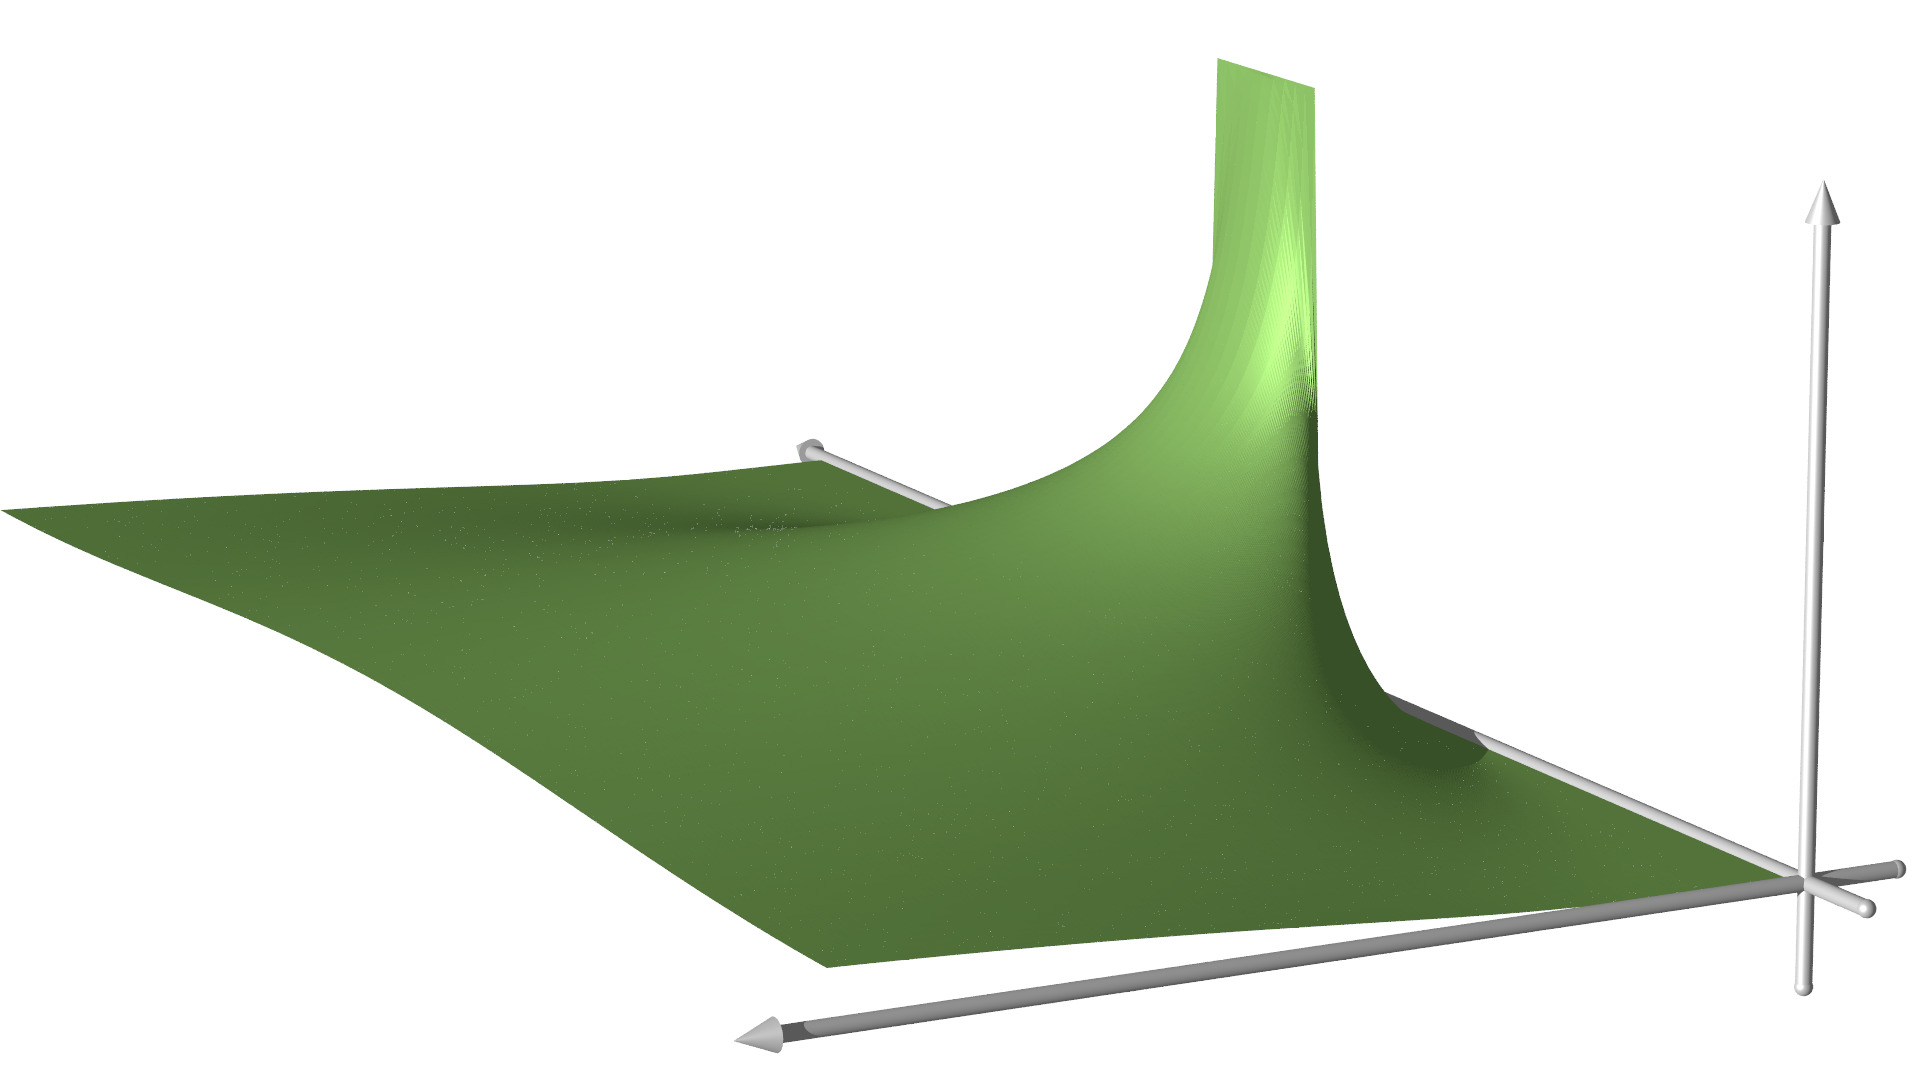
\includegraphics[width=\hsize]{chapters/70-pde/images/implizit.jpg}
\caption{Lösung der Wärmeleitungsgleichung mit dem Rückwärtsverfahren.
\label{buch:pde:waerme:figure:rueckwaerts}}
\end{figure}

\subsubsection{Crank-Nicholson-Verfahren}
Für das Crank-Nicholson-Verfahren sind die Gleichungen am Rand
des Intervals
\begin{align*}
-cu_{0,k+1}+2(1+c)u_{1,k+1}-cu_{2,k+1}
&=
cu_{0k}+2(1-c)u_{1k}+cu_{2,k}
\\
(2+c)u_{1,k+1}-cu_{2,k+1}
&=
(2-c)u_{1k}+cu_{2,k},
\end{align*}
so dass die Matrixgleichung
\begin{gather*}
Cu_{k+1}
=
\begin{pmatrix}
 2+c &  -c  &      &      &      &      &      \\
  -c &2(1+c)&  -c  &      &      &      &      \\
     &   -c &2(1+c)&  -c  &      &      &      \\
     &      &\ddots&\ddots&\ddots&      &      \\
     &      &      &\ddots&\ddots&\ddots&      \\
     &      &      &      &   -c &2(1+c)&  -c  \\
     &      &      &      &      &  -c  &  2+c
\end{pmatrix}
u_{k+1}
\qquad
\qquad
\qquad
\\
\qquad
\qquad
\qquad
=
\begin{pmatrix}
 2-c &   c  &      &      &      &      &      \\
   c &2(1-c)&   c  &      &      &      &      \\
     &    c &2(1-c)&   c  &      &      &      \\
     &      &\ddots&\ddots&\ddots&      &      \\
     &      &      &\ddots&\ddots&\ddots&      \\
     &      &      &      &    c &2(1-c)&   c  \\
     &      &      &      &      &   c  &  2-c
\end{pmatrix}
u_k
=
Du_k
\end{gather*}
wird.
Daraus erhält man als Iterationsverfahren:
\[
u_{k+1} = C^{-1}Du_k.
\]
Das Eigenwertspektrum (Abbildung~\ref{buch:pde:waerme:cranknicholson:spektrum})
hat wieder einen einfachen Eigenwert $1$,
alle anderen Eigenwerte haben Betrag $<1$, das Verfahren ist
konvergent obwohl der Spektralradius exakt $1$ ist.
\begin{figure}
\centering
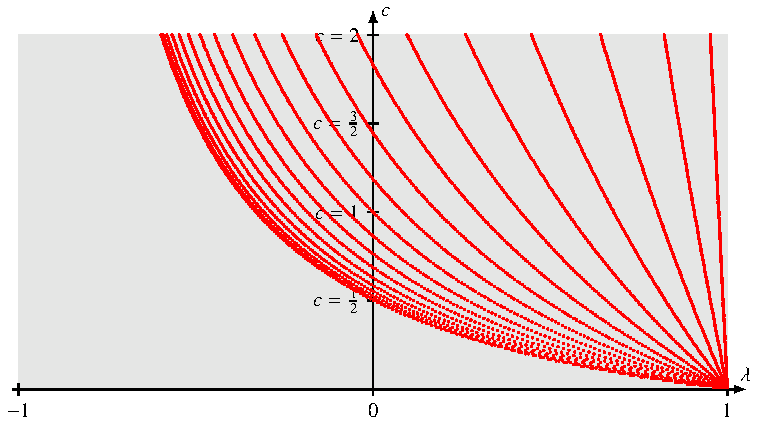
\includegraphics{chapters/70-pde/images/cnspektrum.pdf}
\caption{Das Eigenwertspektrum des Crank-Nicholson-Verfahrens zeigt
einen einzelnen Eigenwert $1$ 
\label{buch:pde:waerme:cranknicholson:spektrum}}
\end{figure}
\begin{figure}
\centering
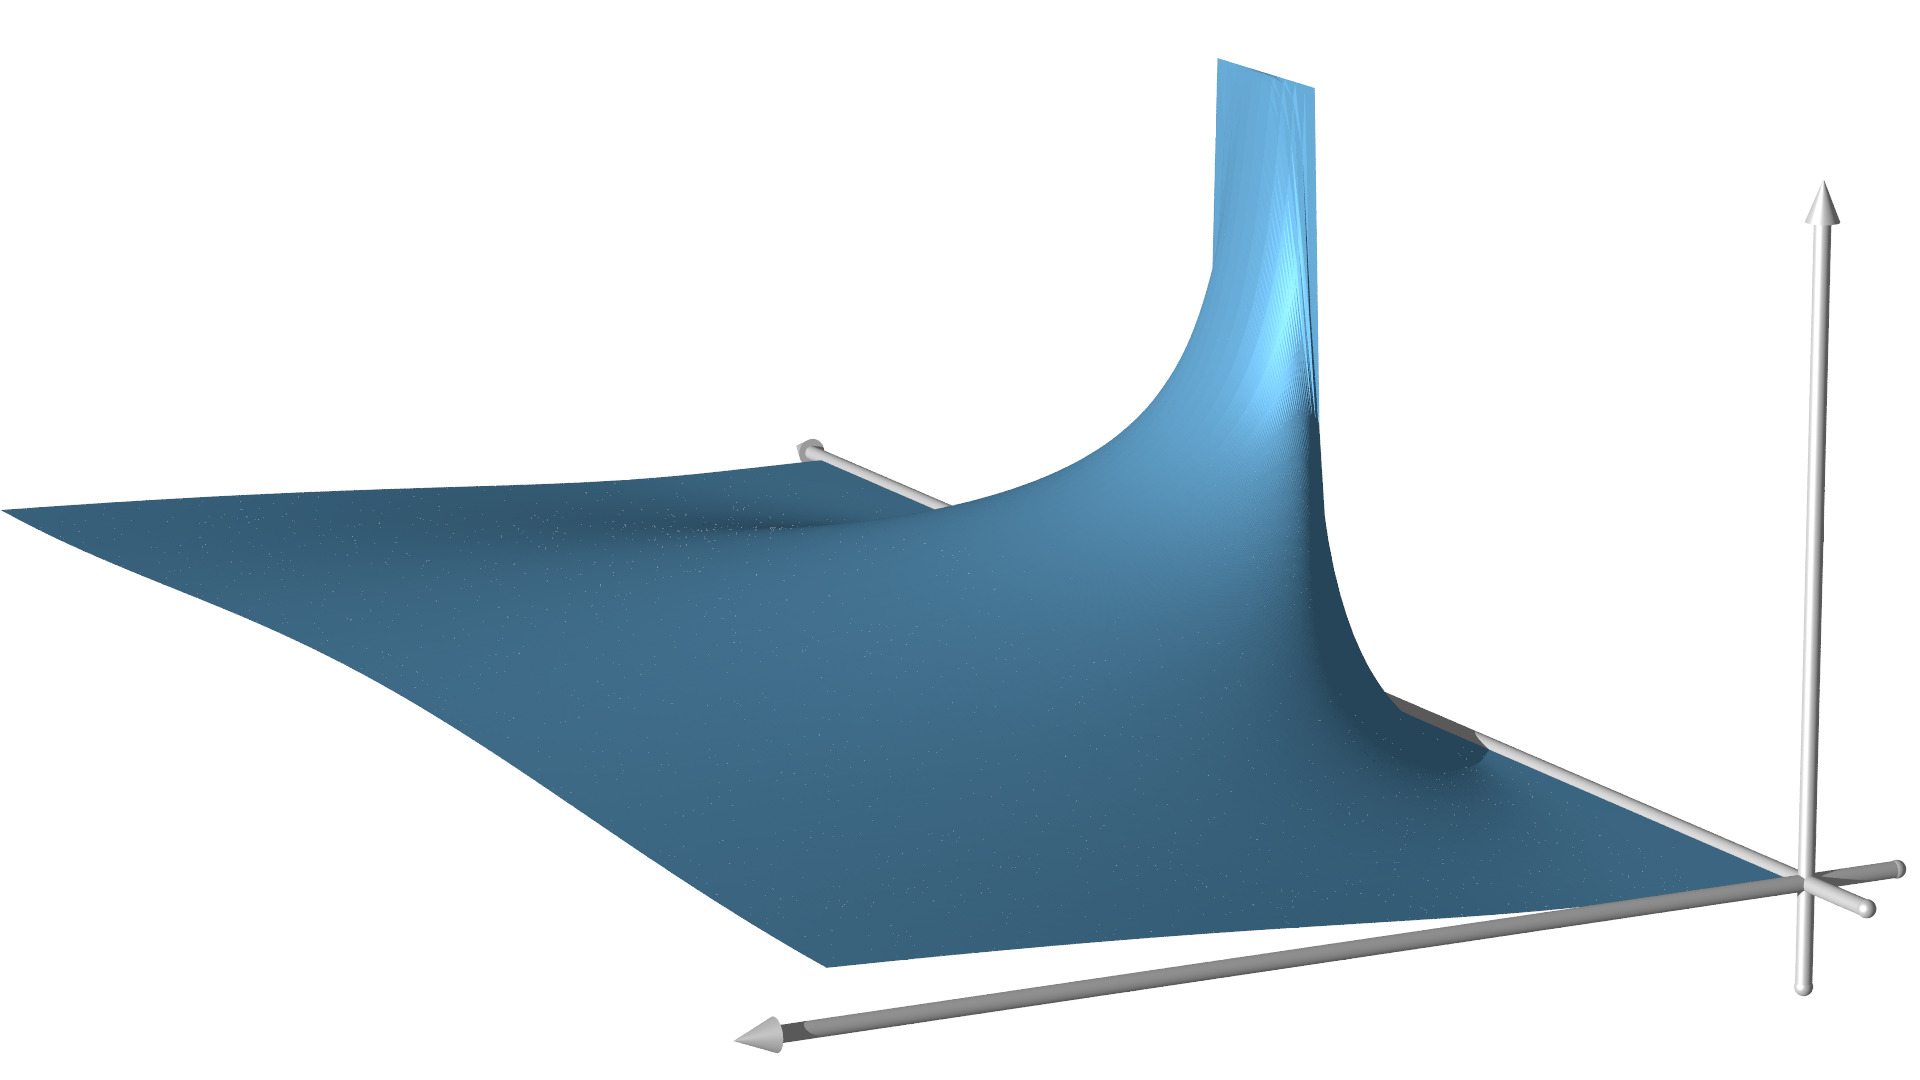
\includegraphics[width=\hsize]{chapters/70-pde/images/cranknicholson.jpg}
\caption{Lösung der Wärmeleitungsgleichung mit dem Crank-Nicholson-Verfahren
\label{buch:pde:waerme:figure:cranknicholson}}
\end{figure}

\begin{figure}
\centering
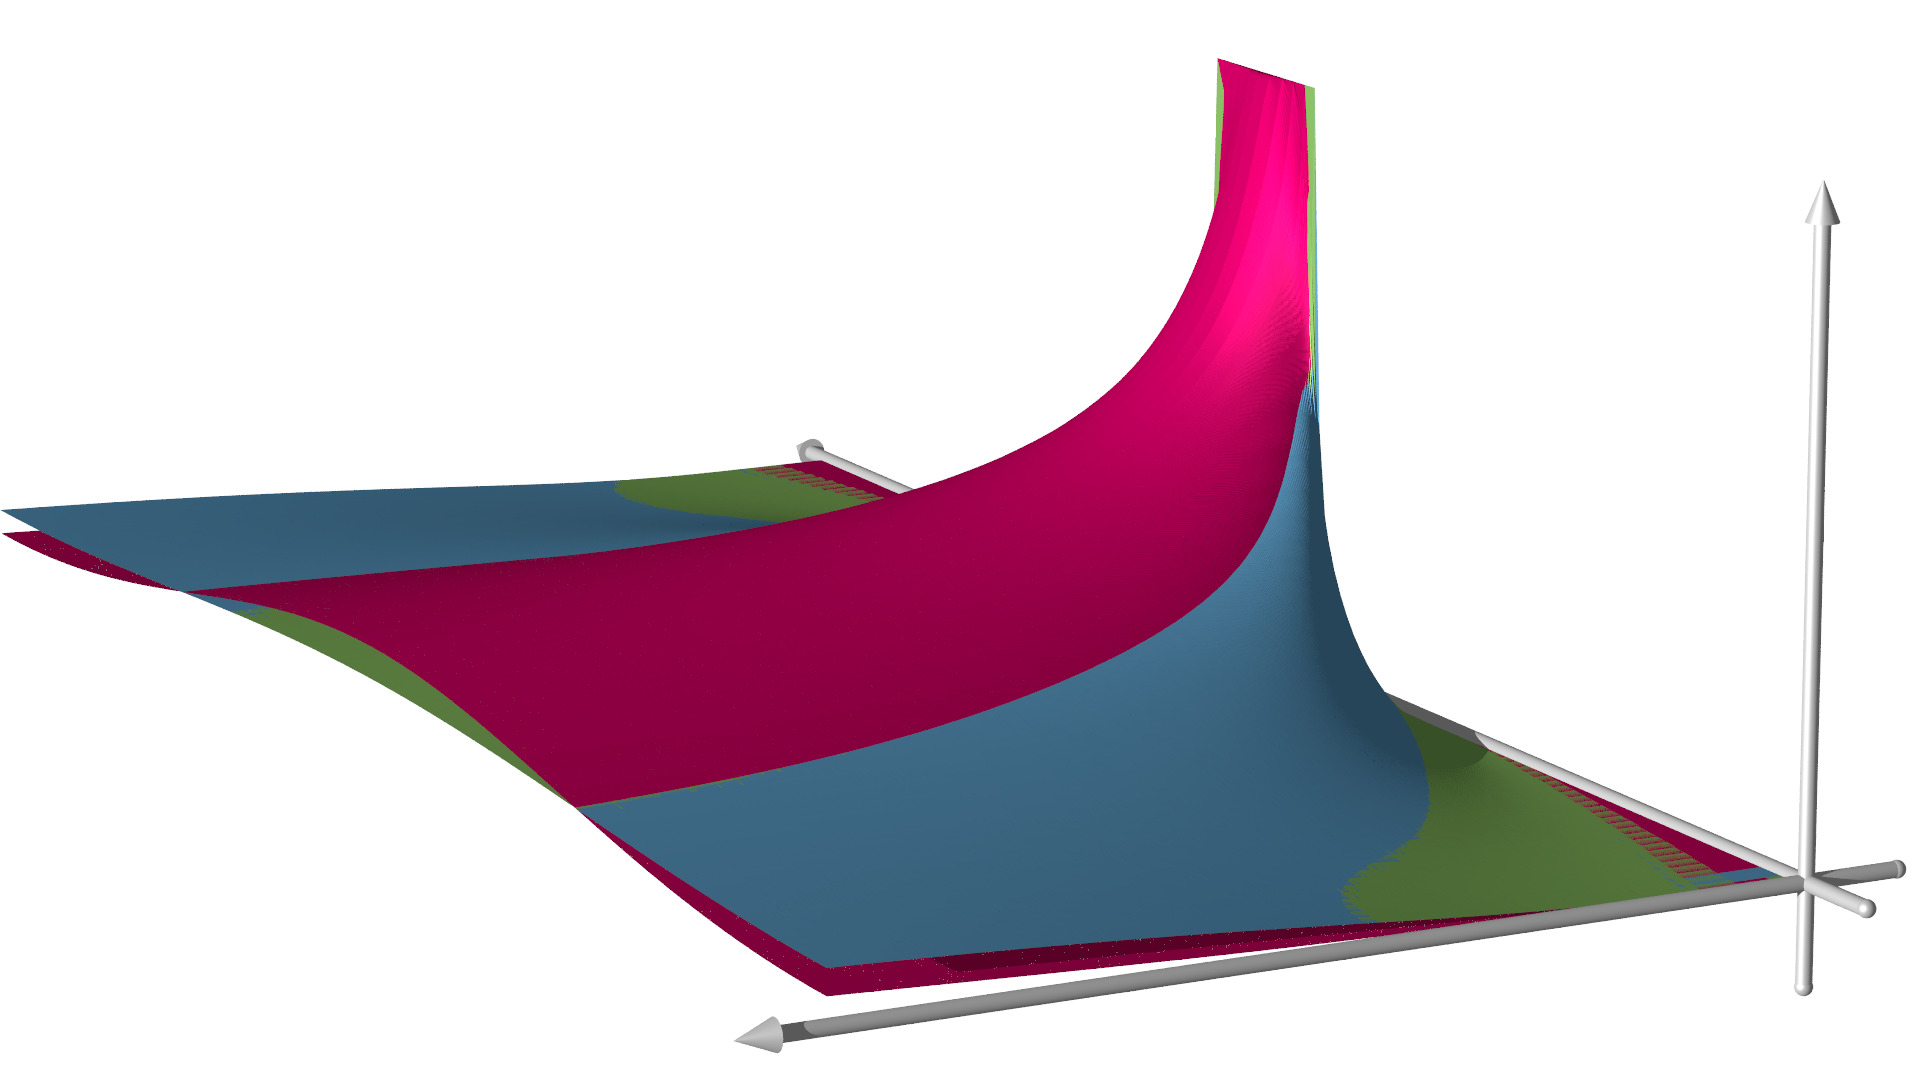
\includegraphics[width=\hsize]{chapters/70-pde/images/combined.jpg}
\caption{Alle drei Lösungsverfahren liefern ähnliche Lösungen,
doch das Euler-Verfahren (rot) weicht stark von den beiden anderen
Verfahren ab.
Das Rückwärts-Verfahren und das Crank-Nicholson-Verfahren stimmen
weitgehend überein.
\label{buch:pde:waerme:figure:combined}}
\end{figure}
In Abbildung~\ref{buch:pde:waerme:figure:combined} sind die drei
Lösungen im gleichen Graphen dargestellt. 
Die Lösung des Euler-Verfahrens weicht stark von den anderen Verfahren ab.
Die Wärmeleitungsgleichung hat Lösungen, bei denen sich Wärme mit
unendlicher Geschwindigkeit ausbreitet.
Im Euler-Verfahren kann sich ein Temperatursprung nur um $h_x$ in
jeder Iteration ausbreiten, also maximal mit der Geschwindigkeit $h_x/h_t$.
Daher verhält sich das Euler-Verfahren so, wie wenn die Wärmeleitfähigkeit
reduziert wäre, was zu dem ausgeprägteren Buckel der Euler-Lösung
führt.



%
% stabilitaet.tex -- Computational mode
%
% (c) 2020 Prof Dr Andreas Müller, Hochschule Rapperswio
%
\subsection{Stabilität und Computational Mode
\label{pde:subsection:stabilitaet}}
In der Diskussion des Wärmeleitungsproblems haben wir für die Zeitableitung
nicht versucht, symmetrische Differenzen zu verwenden.
Tatsächlich gibt es einen wichtigen Grund dafür, der in diesem Abschnitt
untersucht werden soll.
Es wird sich zeigen, dass symmetrische Differenzen zusätzliche instabile
Lösungen erzeugen können, die nichts mit realen Lösungen der
Differentialgleichung zu tun haben.
Dieser sogenannte {\em Computational Mode}
\index{Computational Mode}
führt auf nutzlose Resultate und dürfte mit ein Grund für die Misserfolge
von Lewis Fry Richardson in seinen Pionierversuchen zur numerischen
Wettervorhersage gewesen sein
\cite{buch:richardson}.

\subsubsection{Vorwärtsdifferenzen}
Zur Illustration des Problem verwenden wir die einfache Differentialgleichung
\[
y' = -y,\quad y(0)=y_0
\]
welche die wohlbekannte Lösung $y(x)=y_0e^{-x}$ hat.
Zur Diskretisation verwenden wir die Gitterpunkte $x_i=ih$, $i\in\mathbb Z$
und versuchen die Werte $y_i = y(x_i)$ zu berechnen.
Diskretisation mit Vorwärts-Differenzen führt auf 
\[
y'(x_i) \approx \frac{y_{i+1}-y_i}{h} = -y(x_i) = -y_i
\quad\Rightarrow\qquad
y_{i+1} = y_u-hy_i = (1-h)y_i.
\]
Damit kann man die Lösung als 
\[
y_i = y_0(1-h)^i
\]
schreiben.
Wählt man $h=x/n$, dann liefert diese Approximation
\[
y(x) = y_0\biggl(1-\frac{x}n\biggr)^n 
\to
y_0e^{-x}
\]
für $n\to\infty$.
Dieses Verfahren konvergiert also, wenn auch nicht besonders schnell,
da das Euler-Verfahren nur ein Verfahren erster Ordnung ist.

\subsubsection{Symmetrische Differenzen}
Eine Schwierigkeit der Verwendung von Vorwärts-Differenzen ist, dass
die Vorwärts-Differenz eher eine Approximation für $y'(x_i+h/2)$ ist,
nicht für $y'(x_i)$.
Wie früher gezeigt wurde, können symmetrische Differenzen die Ableitung
im Punkt $x_i$ besser darstellen.
Die zugehörige Differenzengleichung wird jetzt
\[
y'(x_i)
=
\frac{y_{i+1}-y_{i-1}}{2h}
=
-y(x_i)
=
-y_i
\qquad\Rightarrow\qquad
y_{i+1}+2hy_i-y_{i-1}=0.
\]
Ein Potenzansatz $x_i=\lambda^i$ liefert die charakteristische Gleichung
\[
\lambda^{i+1} +2h\lambda^i -\lambda^{i-1}
=
\lambda^{i-1}(\lambda^2 + 2h\lambda -1)
=
0
\]
mit den Lösungen
\[
\lambda_\pm = -h \pm \sqrt{h^2+1}.
\]
Die Quadratwurzel kann in die Taylor-Reihe
\[
\sqrt{1+h^2}
\approx
1 + \frac{h^2}2 + O(h^4)
\]
entwickelt werden.
Es folgt, dass $\lambda$-Wert für das positive Vorzeichen
\[
\lambda_+
=
-h+\sqrt{h^2+1}
\approx
1-h+\frac{h^2}{2}+\dots
<
1
\]
kleiner als $1$ ist, insbesondere ist die Folge $\lambda_+^i$ monoton fallend.

Verwenden wir wieder die Schrittweite $h=x/n$, dann ist
\[
y_i
=
y_0 \lambda_+^i
=
y_0 \biggl(1-h+\frac{h^2}2\biggr)^n
=
y_0\biggl(1-\frac{x}n + o(h)\biggr)^n
\to
y_0e^{-x}
\]
für $n\to\infty$, die Lösung für positives Vorzeichen liefert also genau
die gleiche Lösung, die wir bereits mit Vorwärtsdifferenzen gefunden haben.

Die zweite Lösung der charakteristischen Gleichung mit dem negativen
Vorzeichen ist
\[
\lambda_-
=
-\frac{h}2 - \sqrt{\frac{h^2}{4}+1}
<
-1.
\]
Die Lösungsfolge $\lambda_-^i$ hat alternierende Vorzeichen, aber die 
Beträge $|\lambda_-^i|$ wachsen exponentiell schnell an.
Die Verwendung symmetrischer Differenzen führt also dazu, dass die
Differenzengleichung eine zweite Lösung bekommt, die exponentiell
schnell anwächst.
Diese zweite Lösung heisst der {\em Computational Mode}.
\index{Computational Mode}

\subsubsection{Numerische Anregung des Computational Mode}
Man muss sich fragen, warum man sich über die zweite Lösung überhaupt
Gedanken machen soll, immerhin wird ja für die Lösung der
Differentialgleichung nur die Lösung $\lambda_+$ benötigt.
Der Grund ist, dass bei der Berechnung der Lösung mit Hilfe der
Rekursionsformel
\[
x_{i+1} = x_{i-1}-2hx_i
\]
die zweite Lösung trotzdem auftritt.
Zu zwei aufeinanderfolgenden Werten $y_0$ und $y_1$ kann man mit der
Rekursionsformel alle weiteren Werte berechnen.
Aber selbst wenn man $y_1 = \lambda+y_0$ setzt, wird die numerische
Rechnung Rundungsfehler einführen, so dass der Wert $y_1$, der für die
Rekursion verwendet wird, nicht mit dem exakten Wert $\lambda_+y_0$
übereinstimmt.
Wir nehmen an, dass dieser Rundungsfehler $\delta$ der einzige
Fehler ist, der im Laufe der Berechnung eingeführt wird.
Wir müssen also die exakte Lösung für die Startwerte $y_0$ und
$\lambda_+y_0+\delta$ bestimmen.
Es sind also Koeffizienten $a_\pm$ zu finden mit
\begin{align*}
a_+ + a_- &= y_0 \\
a_+\lambda_+ + a_-\lambda_-&=y_0\lambda_++\delta
\end{align*}
Subtrahiert man das $\lambda_+$-fache der ersten Gleichung von der
zweiten Gleichung, erhält man
\[
a_-(\lambda_-\lambda_+)=\delta
\qquad\Rightarrow\qquad
a_- = \frac{\delta}{\lambda_--\lambda_+} = -\frac{\delta}{h}.
\]
Es folgt, dass selbst ein einziger minimaler Fehler $\delta$
bei der Berechnung von $y_1$ die Lösung die zweite Lösung sichtbar
macht. 

Man kann auch ausrechnen, wie gross $i$ werden muss, bis der
Computational Mode von der gleichen Grössenordnung wie die
gesuchte Lösung geworden ist.
Dieser Fall tritt ein wenn
\[
|y_0\lambda_+^i| < |\delta\lambda_-^i|
\qquad\Rightarrow\qquad
\biggl|
\frac{\lambda_-}{\lambda_+}
\biggr|^i
> \biggl|\frac{y_0}{\delta}\biggr|
\quad\Rightarrow\quad
i
>
\frac{\log |y_0/\delta|}{\log|\lambda_-/\lambda_+|}.
\]
Für kleine Werte von $h$ ist
\[
\log |\lambda_\pm|
=
\log(1\mp h+o(h)) 
\approx
\mp h.
\]
Die Bedingung an $i$ kann man damit mit
\[
i \gtrsim \frac{\log |y_0/\delta|}{2h}
\]
approximieren.
Der $x$-Wert, bei dem der Computational Mode überhand nimmt, ist daher
\[
x \gtrsim h \frac{\log|y_0/\delta|}{2h} = \frac12(\log|y_0|-\log|\delta|)
\]
Für den \texttt{double}-Typ ist $|\delta| \approx 10^{-15}$,
das Verfahren ist also grundsätzlich nicht in der Lage, vernünftige
Resultate für $x>7.5\log 10\approx 17.269$ zu liefern.

\begin{figure}
\centering
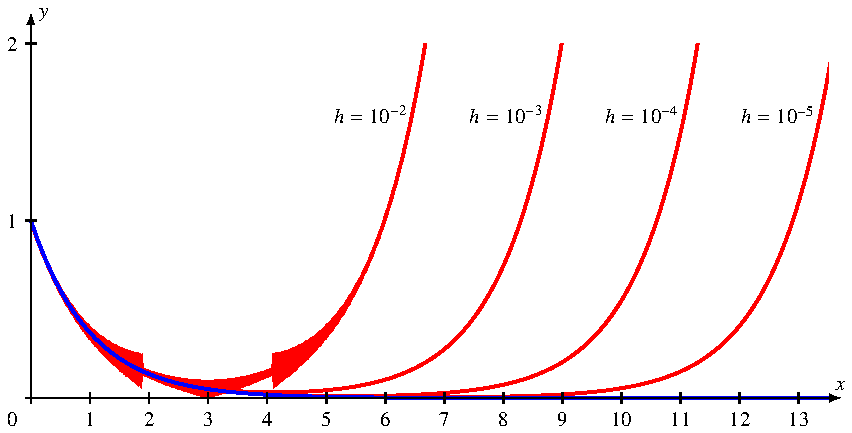
\includegraphics{chapters/70-pde/experiments/computationalmode.pdf}
\caption{Betrag der Lösung der Differentialgleichung $y'=-y$ berechnet
mit Hilfe symmetrischer Differenzen.
\label{buch:pde:cm:fig}}
\end{figure}
Die Annahme, der einzige Fehler trete bei der Rundung von $y_1$ auf,
ist natürlich viel zu optimistisch.
In Wahrheit tritt in jedem Schritt ein Fehler auf, so dass der 
Computational Mode schon viel früher angeregt wird.
In Abbildung~\ref{buch:pde:cm:fig} ist der Betrag der Lösung
für verschiedene Schrittweiten $h$ gezeigt.
Ganz zu Beginn, für $x<1$, scheint die Lösung einigermassen genau dem
theoretisch zu erwartenden Verlauf zu entsprechen.
Dann beginnt jedoch der Computational Mode überhand zu nehmen,
die Lösung wächst exponentiell schnell an und wird unbrauchbar.

Mehr Information zum Computational Mode insbesondere auch zu einer
Filtertechnik, mit der der Computational Mode auch wieder gedämpft
werden kann, ist im Kapitel~\ref{chapter:burgers} zu finden.








